% !TeX spellcheck = en_US
\section{Problem 2}

We are asked to write a Python program that implements steepest descent algorithm for the 1-$S^1$-1 RBF network.
The input function that we want to approximate is 
\[
g(p) = 1 + \sin\left(p\pi/8\right), \quad \text{for} \ p \in \left[-4,4\right]
\]

We select 30 data randomly from that interval and all parameters are initialized as small numbers using \verb|numpy.random.randn| function. It returns a number at the exact specification as needed.

\begin{figure}[htbp]
	\centering
	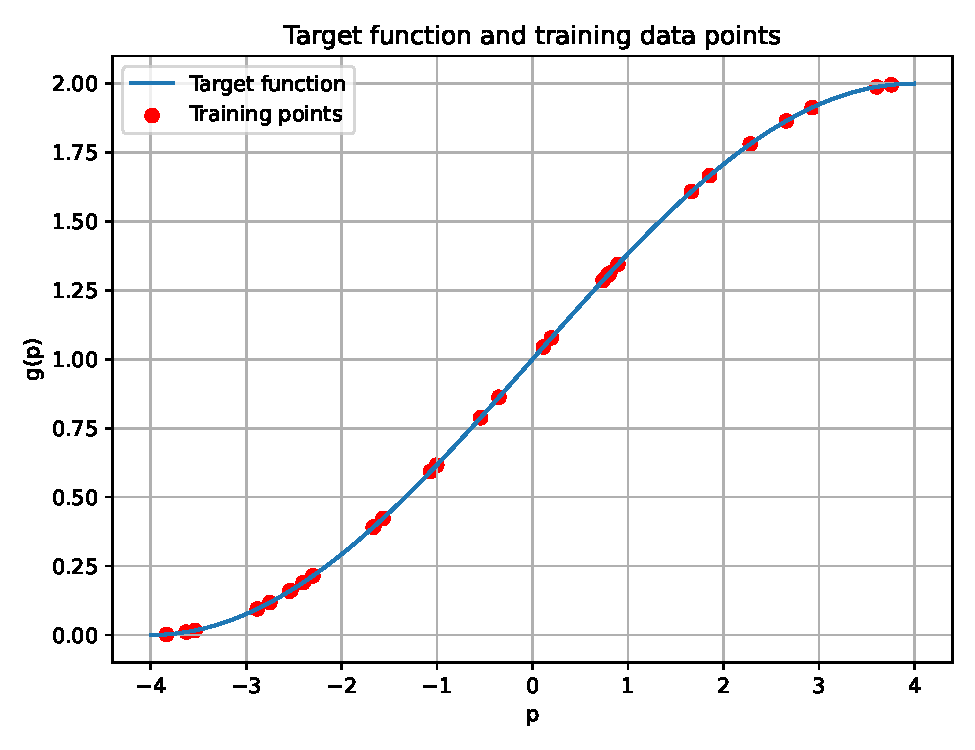
\includegraphics[width=0.6\linewidth]{../Problem 2/prob2_targetFunc_dataPoints.pdf}
	\caption{Input function in the specified area and the randomly assigned train data points.}
\end{figure}

For the randomly assigned data points, we added a custom seed number in order for the results to be comparable but to still use randomness.
The number of centers define the total number of hidden layers in the network.Consequently, training it will affect its accuracy.\\

Every arithmetic operation is done in matrix mode using \verb|np.array| object type for better scalability and automation.
For learning rate values $\alpha$ we used $\left[0.001, 0.005, 0.01\right]$ and for center the values $\left[4, 8, 12, 20\right]$, as suggested. As for the iterations number, we opted for $20\cdot 10^3$ as we didn't want any possible bottleneck in the epoch number.\\

\begin{figure}[htbp]
	\centering
	\begin{subfigure}{0.33\linewidth}
		\centering
		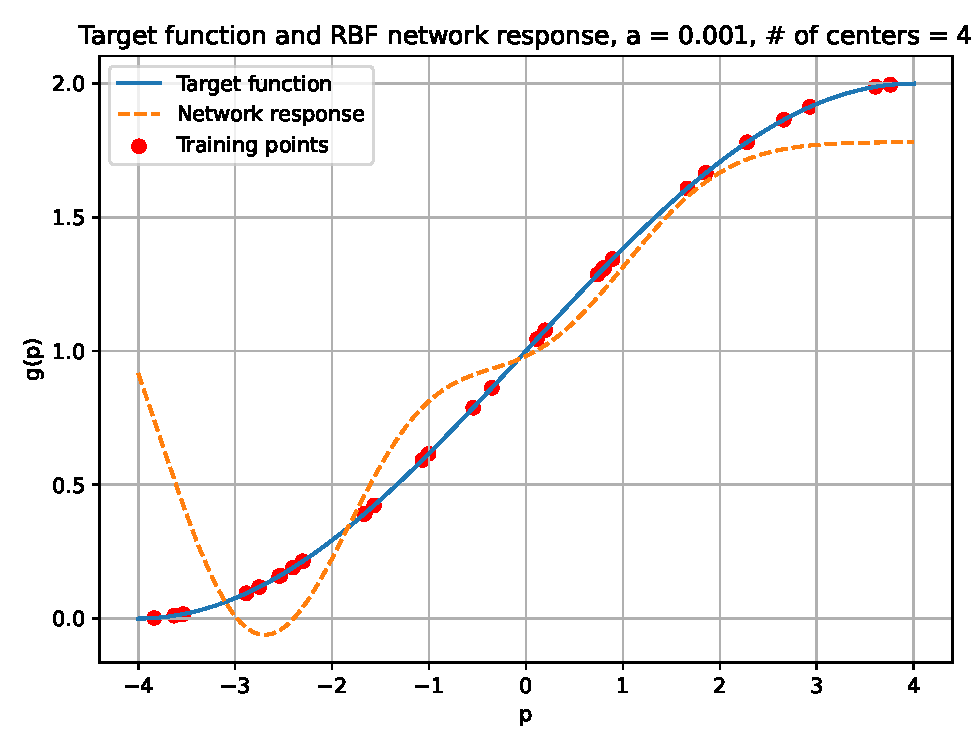
\includegraphics[width=\linewidth]{../Problem 2/prob2_response_a_0.001_Cnum_4.pdf}
		\caption{$a=0.001$}
	\end{subfigure}\hfill
	\begin{subfigure}{0.33\linewidth}
		\centering
		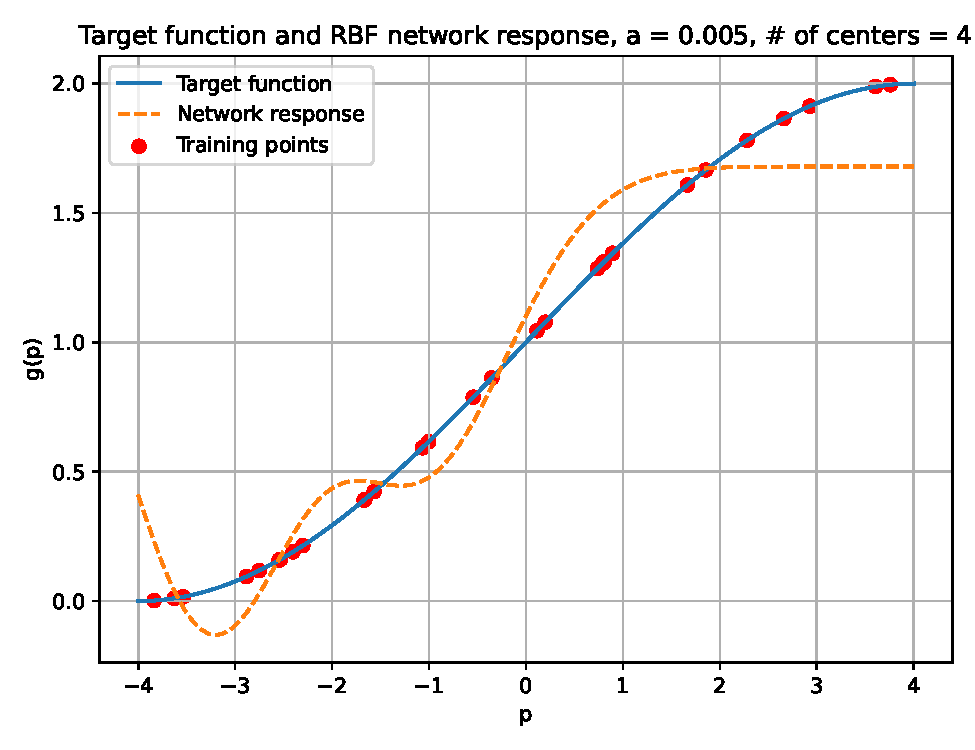
\includegraphics[width=\linewidth]{../Problem 2/prob2_response_a_0.005_Cnum_4.pdf}
		\caption{$a=0.005$}
	\end{subfigure}\hfill
	\begin{subfigure}{0.33\linewidth}
		\centering
		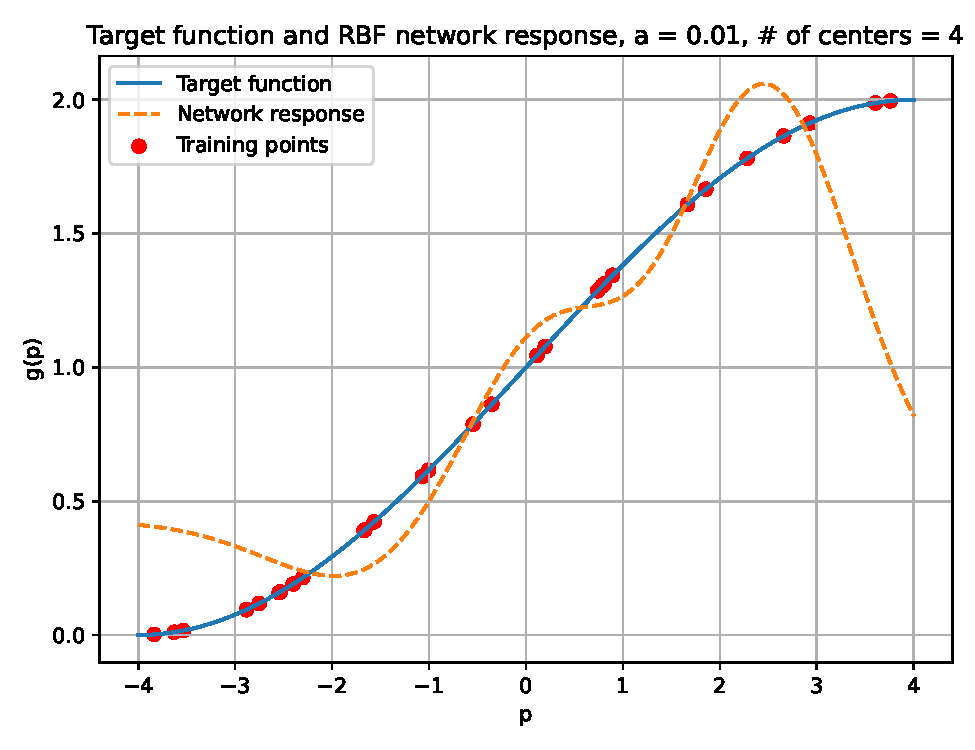
\includegraphics[width=\linewidth]{../Problem 2/prob2_response_a_0.01_Cnum_4.pdf}
		\caption{$a=0.01$}
	\end{subfigure}\hfill
	\caption{Input function approximation with number of centers $=4$.}
	\label{fig:prob2_response_4}
\end{figure}

\begin{figure}[htbp]
	\centering
	\begin{subfigure}{0.33\linewidth}
		\centering
		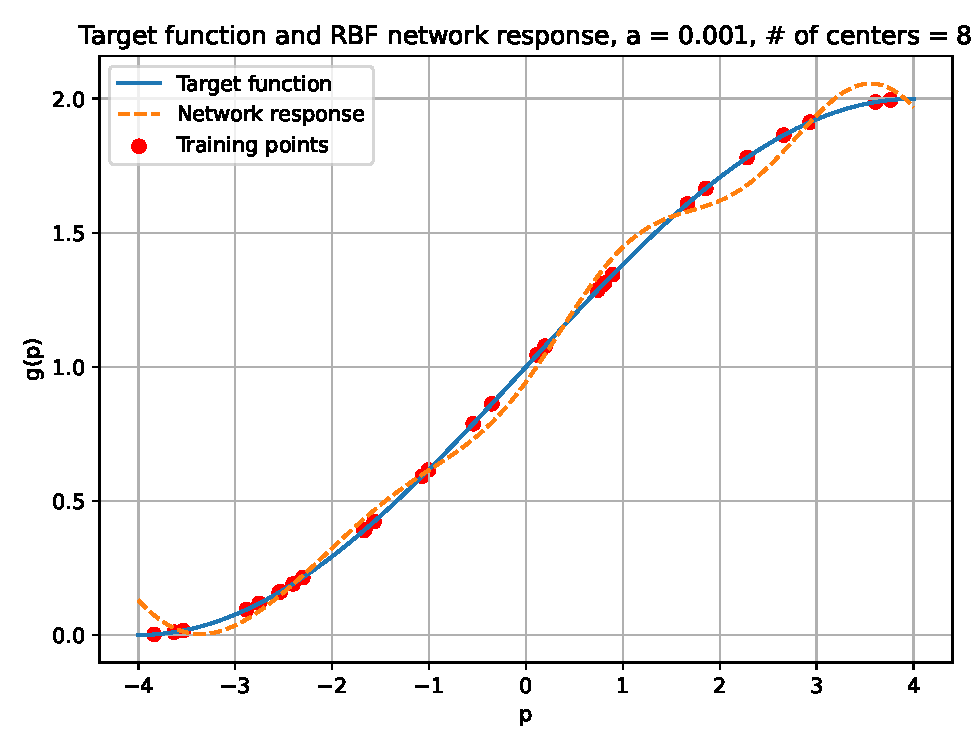
\includegraphics[width=\linewidth]{../Problem 2/prob2_response_a_0.001_Cnum_8.pdf}
		\caption{$a=0.001$}
	\end{subfigure}\hfill
	\begin{subfigure}{0.33\linewidth}
		\centering
		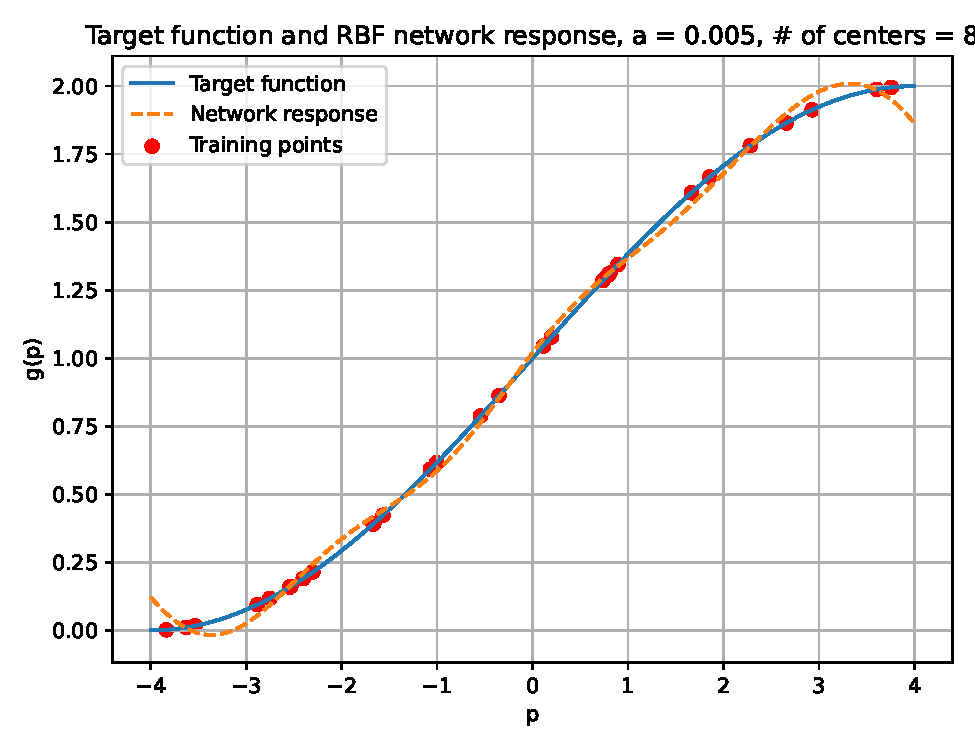
\includegraphics[width=\linewidth]{../Problem 2/prob2_response_a_0.005_Cnum_8.pdf}
		\caption{$a=0.005$}
	\end{subfigure}\hfill
	\begin{subfigure}{0.33\linewidth}
		\centering
		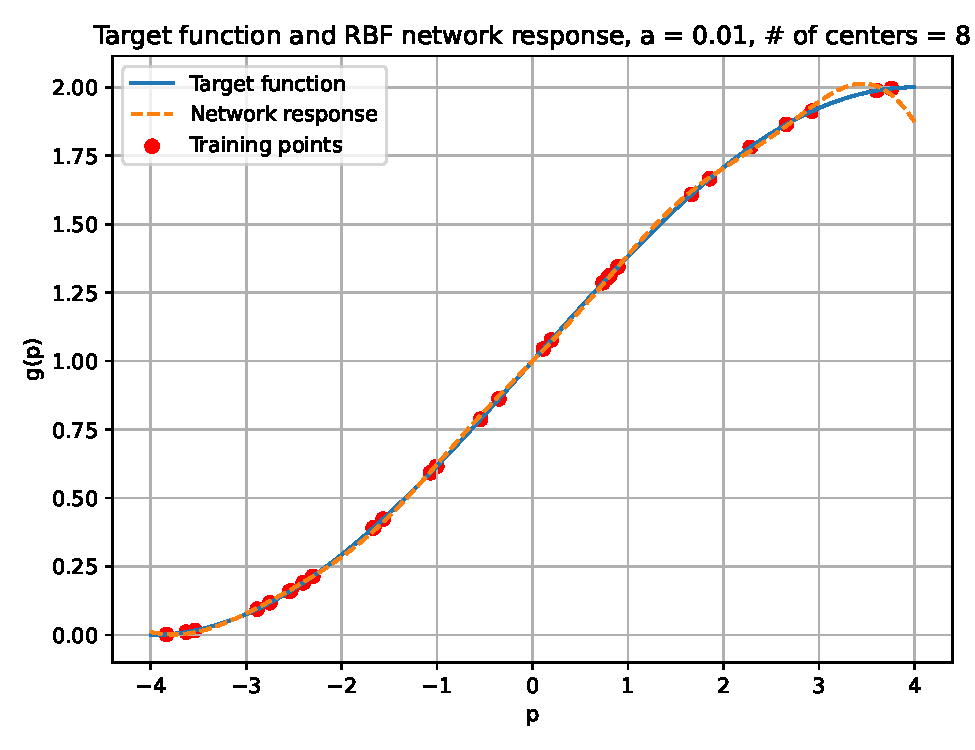
\includegraphics[width=\linewidth]{../Problem 2/prob2_response_a_0.01_Cnum_8.pdf}
		\caption{$a=0.01$}
	\end{subfigure}\hfill
	\caption{Input function approximation with number of centers $=8$.}
	\label{fig:prob2_response_8}
\end{figure}

\begin{figure}[htbp]
	\centering
	\begin{subfigure}{0.33\linewidth}
		\centering
		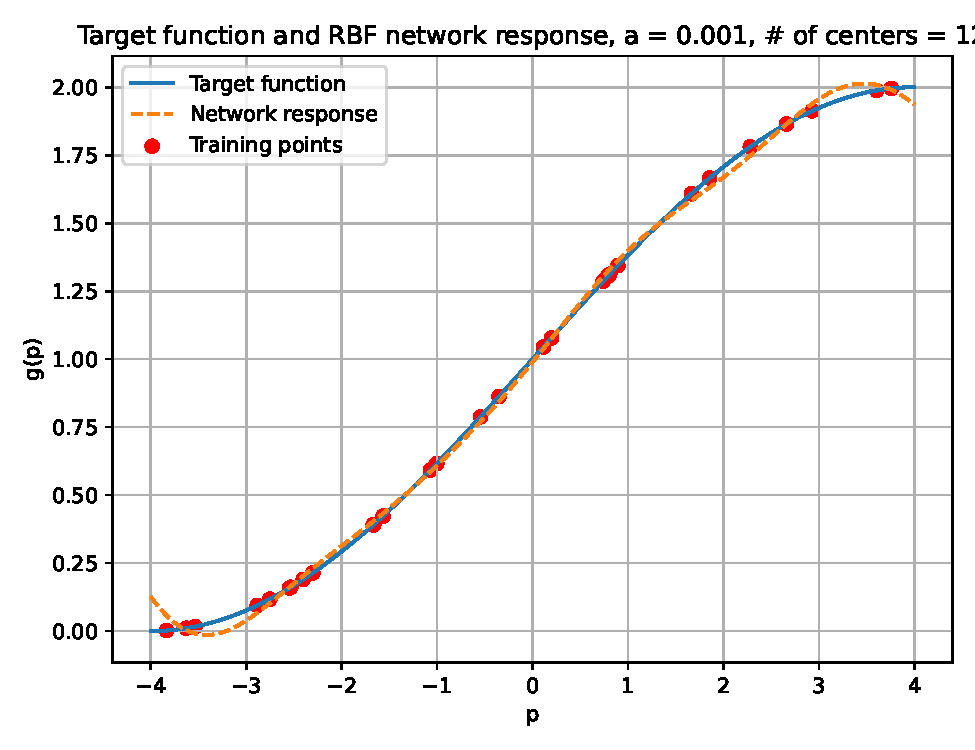
\includegraphics[width=\linewidth]{../Problem 2/prob2_response_a_0.001_Cnum_12.pdf}
		\caption{$a=0.001$}
	\end{subfigure}\hfill
	\begin{subfigure}{0.33\linewidth}
		\centering
		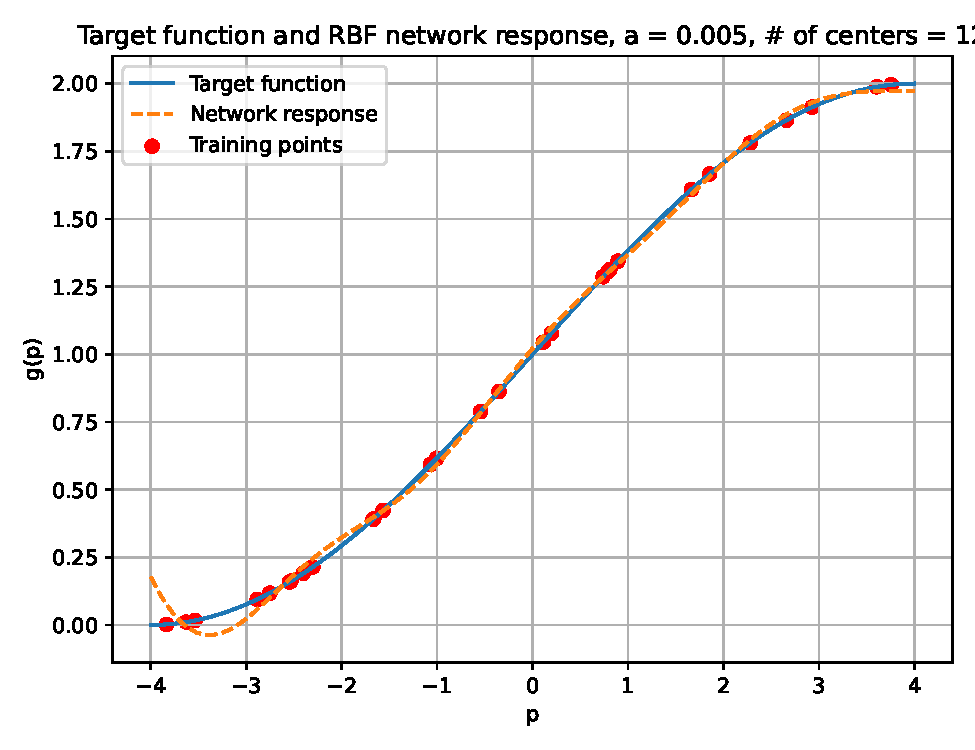
\includegraphics[width=\linewidth]{../Problem 2/prob2_response_a_0.005_Cnum_12.pdf}
		\caption{$a=0.005$}
	\end{subfigure}\hfill
	\begin{subfigure}{0.33\linewidth}
		\centering
		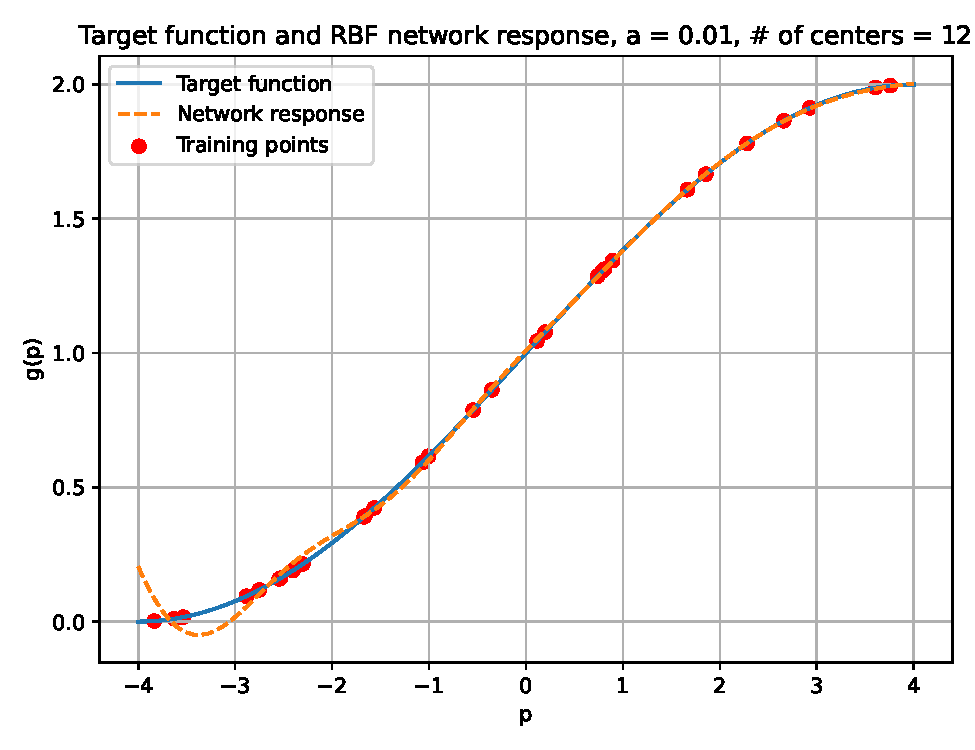
\includegraphics[width=\linewidth]{../Problem 2/prob2_response_a_0.01_Cnum_12.pdf}
		\caption{$a=0.01$}
	\end{subfigure}\hfill
	\caption{Input function approximation with number of centers $=12$.}
	\label{fig:prob2_response_12}
\end{figure}

\begin{figure}[htbp]
	\centering
	\begin{subfigure}{0.33\linewidth}
		\centering
		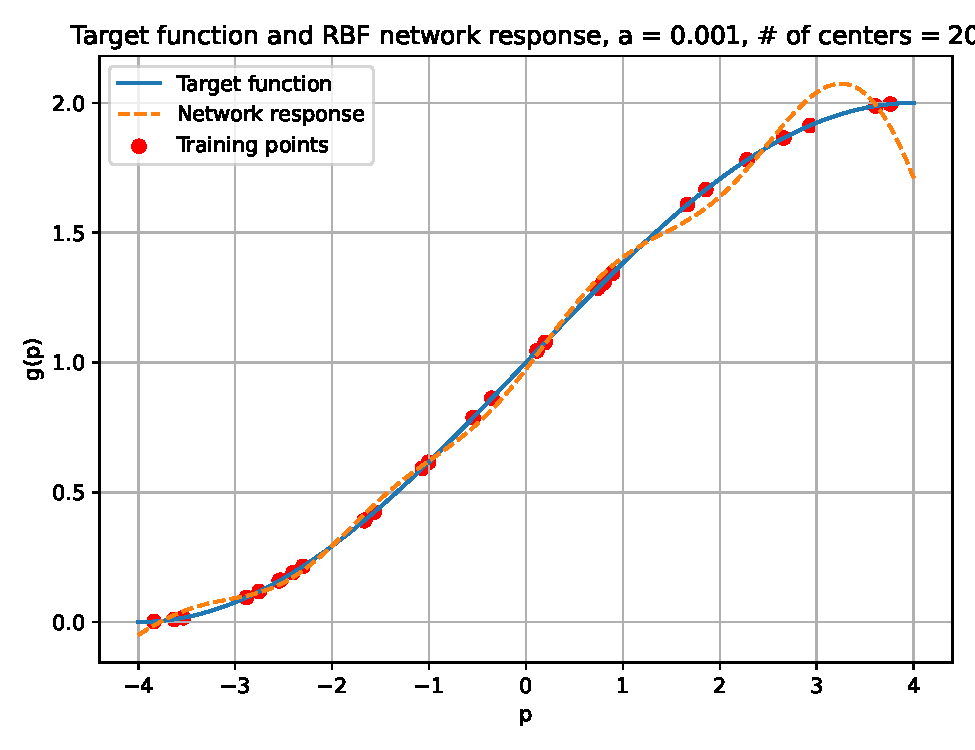
\includegraphics[width=\linewidth]{../Problem 2/prob2_response_a_0.001_Cnum_20.pdf}
		\caption{$a=0.001$}
	\end{subfigure}\hfill
	\begin{subfigure}{0.33\linewidth}
		\centering
		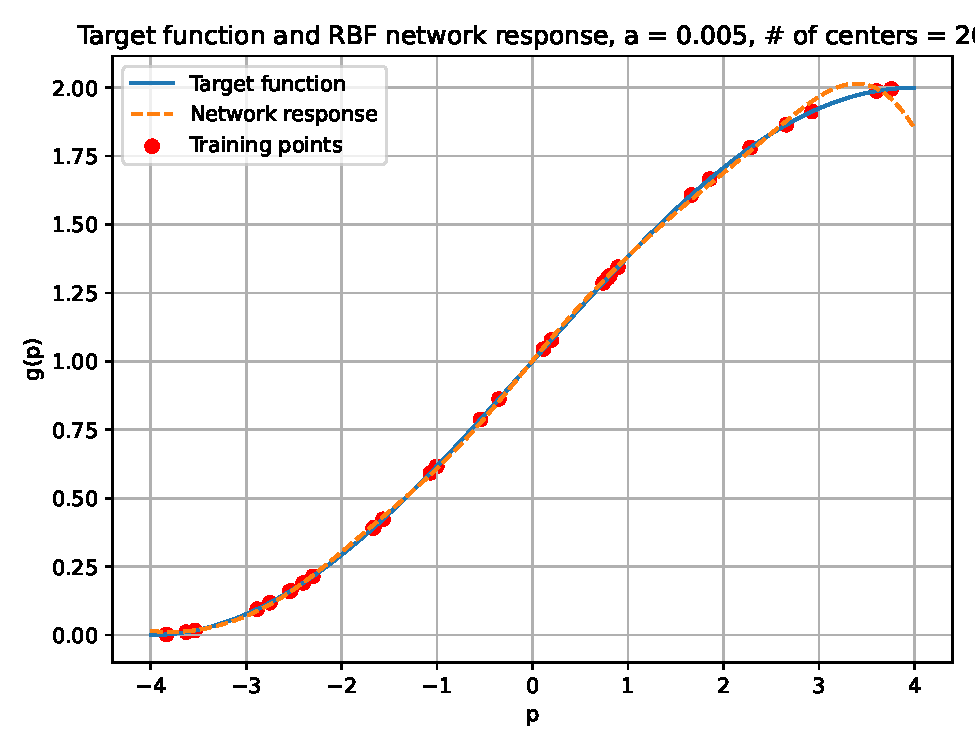
\includegraphics[width=\linewidth]{../Problem 2/prob2_response_a_0.005_Cnum_20.pdf}
		\caption{$a=0.005$}
	\end{subfigure}\hfill
	\begin{subfigure}{0.33\linewidth}
		\centering
		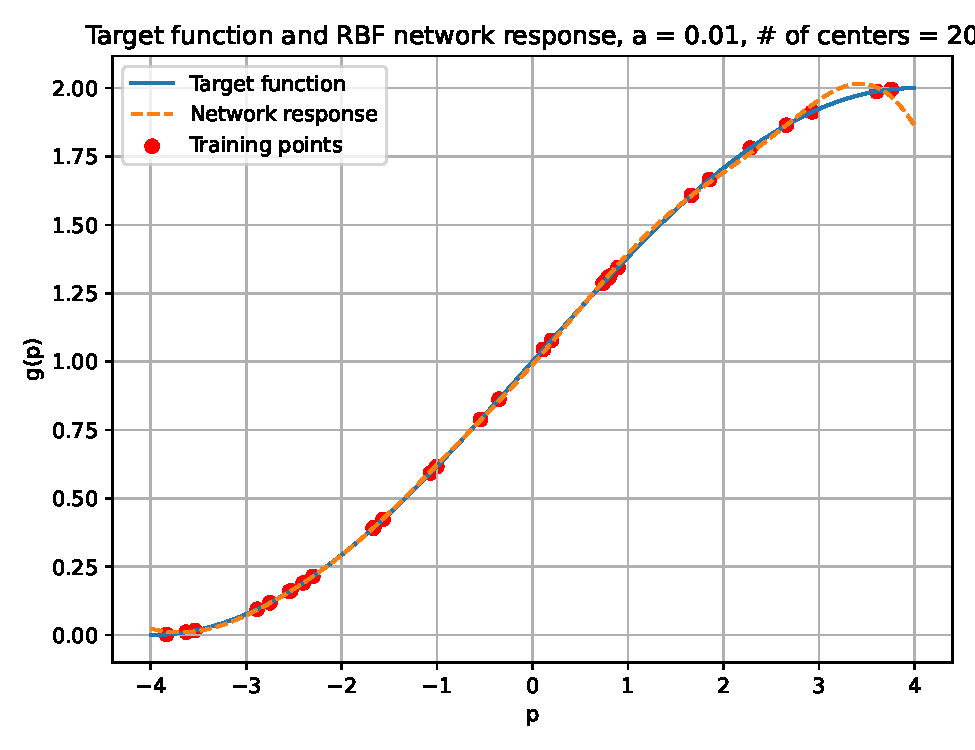
\includegraphics[width=\linewidth]{../Problem 2/prob2_response_a_0.01_Cnum_20.pdf}
		\caption{$a=0.01$}
	\end{subfigure}\hfill
	\caption{Input function approximation with number of centers $=20$.}
	\label{fig:prob2_response_20}
\end{figure}

In figures \ref{fig:prob2_response_4}, \ref{fig:prob2_response_8}, \ref{fig:prob2_response_12} and \ref{fig:prob2_response_20} we can see the output of the neural network for each $\alpha$ and number of center (\textit{hidden layers}).

Firstly, let's consider the impact of the number of centers. As we increase hat number from 4 to 8, 12, and then 20, the output dynamics undergo a notable transformation. With a smaller number of centers, the network struggles to capture intricate patterns in the data, leading to underfitting.
This can be seen particularly well in figure~\ref{fig:prob2_response_4}, where number of centers is $4$. The network fails to predict the input signal across all data points.
Conversely, increasing the number of centers enables the network to model more complex relationships, reducing the underfitting and improving generalization.
Again, these observations are very clear from the first change in the number of centers, from $4$ to $8$. The latter network has a smaller error across all data points when compared to the input signal. This increase of quality is not observed only in this increase of center numbers, but to all increases.

Next, let's delve into the impact of the learning rate on the RBF layer's output. A higher learning rate accelerates the convergence of the training process, enabling the model to reach a satisfactory solution faster.
However, a learning rate that is too high might lead to oscillations or divergence, hindering the convergence process.
From our calculations, when $\alpha$ is increased above $0.05$, the system is diverging and by a large factor. 
On the other hand, a lower learning rate ensures more cautious updates to the model parameters, reducing the risk of divergence but potentially prolonging the convergence process.
Thus, the output dynamics with different learning rates exhibit variations in convergence speed and possibly final performance, with an optimal learning rate striking a balance between convergence efficiency and stability.
\vspace{3mm}